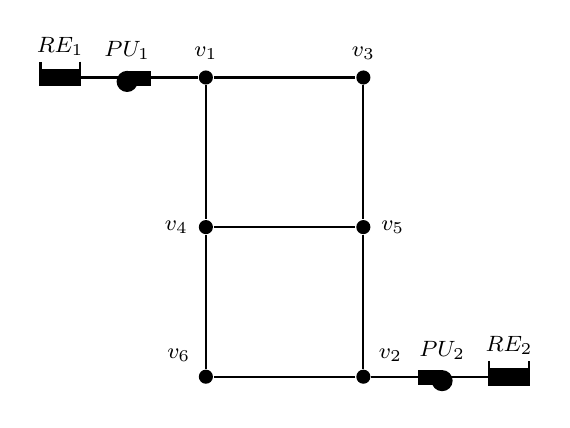
\begin{tikzpicture}[semithick,state/.style ={ draw,shape=circle,scale=0.9}]

\node[circle,fill,inner sep=1.8pt,label=above : \footnotesize$v_1$] (A) at (0,0) {};
\node[circle,fill,inner sep=1.8pt,label=above : \footnotesize$v_3$] (B) at (2,0) {};
\node[circle,fill,inner sep=1.8pt,label= left: \footnotesize$v_4$] (C) at (0,-1.9) {};
\node[circle,fill,inner sep=1.8pt,label= right: \footnotesize$v_5$] (D) at (2,-1.9) {};
\node[circle,fill,inner sep=1.8pt,label= above right: \footnotesize $v_{2}$] (E) at (2,-3.8) {};
\node[circle,fill,inner sep=1.8pt,label= above left: \footnotesize$v_6$] (F) at (0,-3.8) {};

\draw [thick] (A) --  (B) node[above  =0.05 cm] {\footnotesize$$};
\path (A) edge [thick]  node[left  =0.05 cm] {\footnotesize$$} (C);
\path (B) edge [thick] node[right  =0.05 cm] {\footnotesize$$} (D);
\path (C) edge [thick] node[above  =0.05 cm] {\footnotesize$$} (D);
\path (C) edge [thick] node[left  =0.05 cm] {\footnotesize$$} (F);
\path (D) edge [thick] node[right  =0.05 cm] {\footnotesize$$} (E);
\path (E) edge [thick] node[below  =0.05 cm] {\footnotesize$$} (F);



%PU2
\node[circle,fill,inner sep=2.7pt,label= above : \footnotesize $ PU_2$] (I) at (3,-3.85) {};
\draw [thin,fill] (2.7,-3.72) rectangle (3,-3.9);


\begin{scope}[xscale=-1,yscale=1]
%PU1
\node[circle,fill,inner sep=2.7pt,label= above : \footnotesize $ PU_1$] (I) at (3.4-2.4,-2.05+2) {};
\draw [thin,fill] (3.1-2.4,-1.92+2) rectangle (3.4-2.4,-2.1+2);

\end{scope}

\draw [thick](2.1,-3.8) -- (2.7,-3.8);
\draw [thick](-0.1,0) -- (-1.1,0);


\draw [thick](3.1,-3.8) -- (3.6,-3.8);
\draw [thick](-1.1,0) -- (-1.6,0);
\draw [thick](-1.6,0.2) -- (-1.6,-0.1) -- (-2.1,-0.1) -- (-2.1,0.2);
\draw [thick,fill] (-2.1,0.1) rectangle (-1.6,-0.1);
\draw [thick](3.6,-3.6) -- (3.6,-3.9) -- (4.1,-3.9) -- (4.1,-3.6);
\draw [thick,fill] (3.6,-3.7) rectangle (4.1,-3.9);
\node at (-1.85,0.4) {\footnotesize $RE_1$};
\node at (3.85,-3.4) {\footnotesize $RE_2$};
\end{tikzpicture}